
%使用XeLaTeX编译
%版权所有,翻版必究
%本文件由程序自动生成,任何修改将被覆盖
%2019 年 01 月 23 日




\FloatBarrier
\section{
Blend
}\label{c000015s000002}


Blend特效常用属性
如\tablename\ \ref{tb000001}:


%使用XeLaTeX编译
%版权所有,翻版必究
%本文件由程序自动生成,任何修改将被覆盖
%2019 年 01 月 23 日



%表
\begin{longtable}{ccc}

%表头....
\toprule{}类名 
&
分类
&
简介%there must use marginnote ...
\marginnote{\setlength\fboxsep{2pt}\fbox{\footnotesize{\kaishu\tablename\,}\footnotesize{\ref{tb000000}}}}
\\ \midrule 
\endfirsthead

%表尾...
\bottomrule
\caption{ThresholdMask}\label{tb000000} 
\endlastfoot

%重复表头
\toprule{}类名 
&
分类
&
简介
\\ \midrule
\endhead
%重复表尾
\midrule
\endfoot 
Blend & aabbc & cccc \\
BrightnessContrast & aabbc & cccc \\
ColorOverlay & aabbc & cccc \\
Colorize & aabbc & cccc \\
Desaturate & aabbc & cccc \\
GammaAdjust & aabbc & cccc \\
HueSaturation & aabbc & cccc \\
LevelAdjust & aabbc & cccc \\
ConicalGradient & aabbc & cccc \\
LinearGradient & aabbc & cccc \\
RadialGradient & aabbc & cccc \\
Displace & aabbc & cccc \\
DropShadow & aabbc & cccc \\
InnerShadow & aabbc & cccc \\
FastBlur & aabbc & cccc \\
GaussianBlur & aabbc & cccc \\
MaskedBlur & aabbc & cccc \\
RecursiveBlur & aabbc & cccc \\
DirectionalBlur & aabbc & cccc \\
RadialBlur & aabbc & cccc \\
ZoomBlur & aabbc & cccc \\
Glow & aabbc & cccc \\
RectangularGlow & aabbc & cccc \\
OpacityMask & aabbc & cccc \\
ThresholdMask  & aabbc & cccc \\
\end{longtable}
%表





%使用XeLaTeX编译
%版权所有,翻版必究
%本文件由程序自动生成,任何修改将被覆盖
%2019 年 01 月 23 日





混合模式
如\tablename\ \ref{tb000002}
    \footnote{$a$代表foregroundSource,
$b$代表source,
$0$代表黑色,
$1$代表白色,
$v$代表最终结果。}
:


%使用XeLaTeX编译
%版权所有,翻版必究
%本文件由程序自动生成,任何修改将被覆盖
%2019 年 01 月 23 日



%表
\begin{longtable}{ccc}

%表头....
\toprule{}类名 
&
分类
&
简介%there must use marginnote ...
\marginnote{\setlength\fboxsep{2pt}\fbox{\footnotesize{\kaishu\tablename\,}\footnotesize{\ref{tb000000}}}}
\\ \midrule 
\endfirsthead

%表尾...
\bottomrule
\caption{ThresholdMask}\label{tb000000} 
\endlastfoot

%重复表头
\toprule{}类名 
&
分类
&
简介
\\ \midrule
\endhead
%重复表尾
\midrule
\endfoot 
Blend & aabbc & cccc \\
BrightnessContrast & aabbc & cccc \\
ColorOverlay & aabbc & cccc \\
Colorize & aabbc & cccc \\
Desaturate & aabbc & cccc \\
GammaAdjust & aabbc & cccc \\
HueSaturation & aabbc & cccc \\
LevelAdjust & aabbc & cccc \\
ConicalGradient & aabbc & cccc \\
LinearGradient & aabbc & cccc \\
RadialGradient & aabbc & cccc \\
Displace & aabbc & cccc \\
DropShadow & aabbc & cccc \\
InnerShadow & aabbc & cccc \\
FastBlur & aabbc & cccc \\
GaussianBlur & aabbc & cccc \\
MaskedBlur & aabbc & cccc \\
RecursiveBlur & aabbc & cccc \\
DirectionalBlur & aabbc & cccc \\
RadialBlur & aabbc & cccc \\
ZoomBlur & aabbc & cccc \\
Glow & aabbc & cccc \\
RectangularGlow & aabbc & cccc \\
OpacityMask & aabbc & cccc \\
ThresholdMask  & aabbc & cccc \\
\end{longtable}
%表





%使用XeLaTeX编译
%版权所有,翻版必究
%本文件由程序自动生成,任何修改将被覆盖
%2019 年 01 月 23 日





如\filesourcenumbernameone\ \ref{f000052}展
示了Blend的常见用法。
\enlargethispage{1cm}
%begin图片
\begin{figure}[htb] %浮动体 here and top ...
%there must use marginnote ...
\marginnote{\setlength\fboxsep{2pt}\fbox{\footnotesize{\kaishu\figurename\,}\footnotesize{\ref{p000018}}}}\centering %中心对齐
\setlength\fboxsep{0pt}\fbox{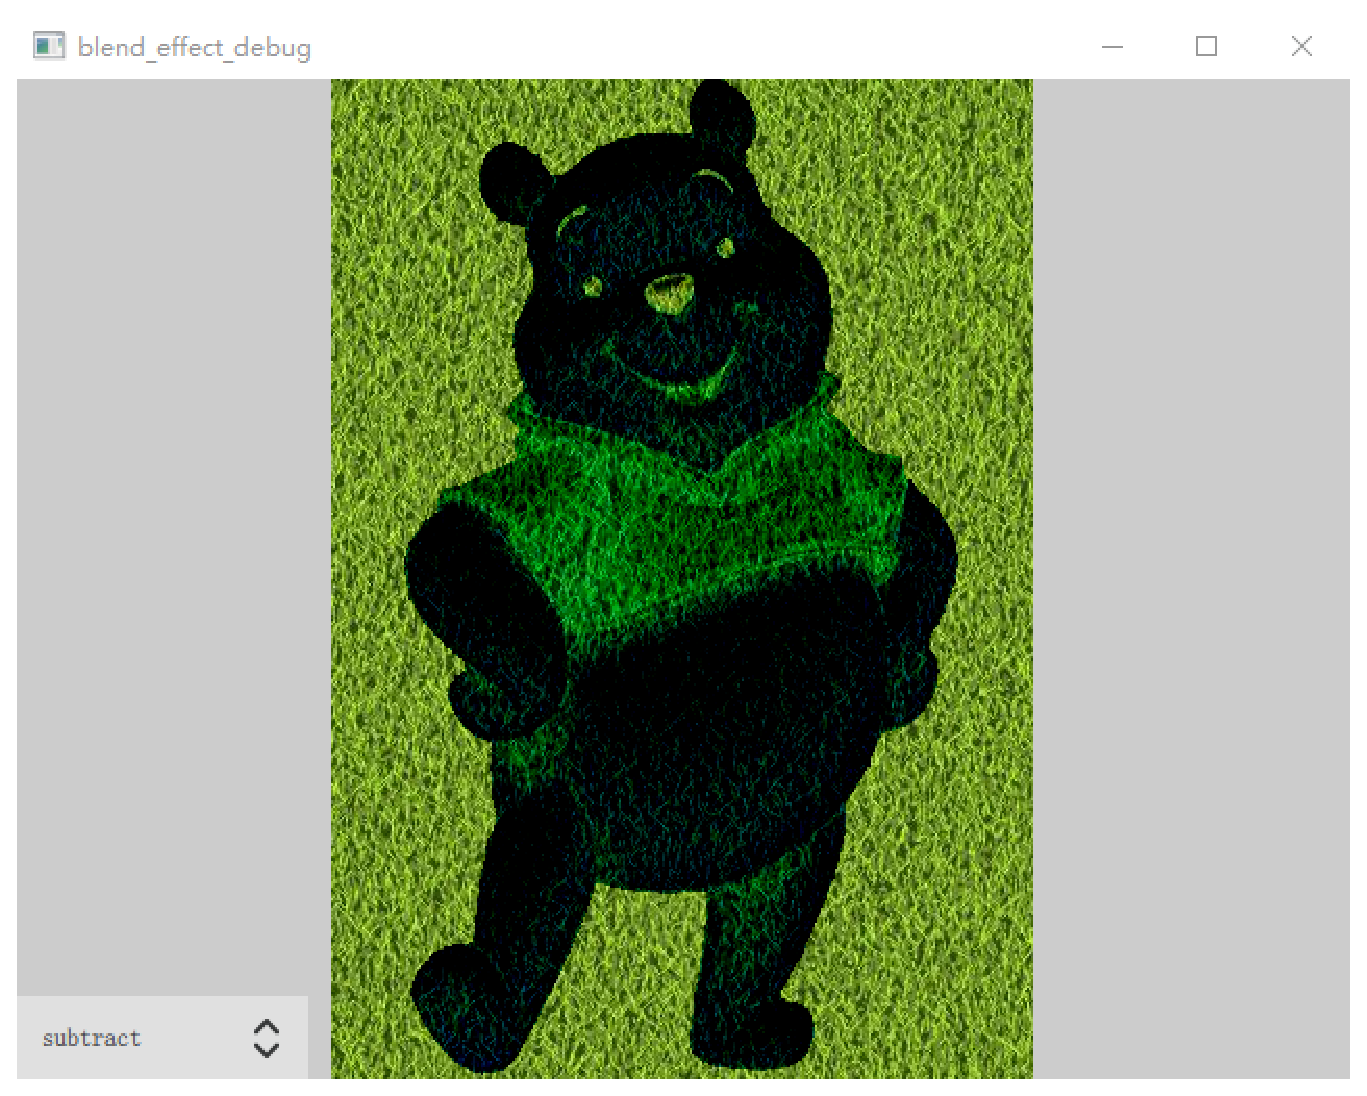
\includegraphics[width=0.95\textwidth]{the_book_image/p000018.eps}} %图片路径
\caption{Blend} %标题
\label{p000018} %索引
\end{figure}

%end图片


%\begin{spacing}{1.0}
\refstepcounter{filesourcenumber}\label{f000052}    %增加源代码编号
\FloatBarrier                                  %强制完成浮动体布局
\begin{thebookfilesourceone}[escapeinside={(*@}{@*)},
caption=GoodLuck,
title=\filesourcenumbernameone \thefilesourcenumber
]
/*blend_effect/main.qml*/
import QtQuick 2.9
import QtGraphicalEffects 1.12

Rectangle {
    id : idRoot
    width: 640;
    height: 480;
    color: Qt.rgba(0.8,0.8,0.8,1);

    Image{
        anchors.fill: idBear;
        source: "grass.jpg"
        fillMode: Image.Tile
        id : idGrass
        visible: false
    }

    Image{
        anchors.centerIn: parent;
        source: "bear.png"
        fillMode: Image.Stretch
        id : idBear
        visible: false
    }

    Blend{
        source: idGrass
        foregroundSource: idBear
        mode: idBlendControl.blendModeComboBox.currentText
        anchors.centerIn: parent;
        width: idBear.width
        height: idBear.height
    }

    BlendControl {
        id : idBlendControl
    }

}(*@\marginpar[\hfill\setlength\fboxsep{2pt}\fbox{\footnotesize{\kaishu\parbox{1em}{\setlength{\baselineskip}{2pt}\filesourcenumbernameone}}\footnotesize{\thefilesourcenumber}}]{\setlength\fboxsep{2pt}\fbox{\footnotesize{\kaishu\parbox{1em}{\setlength{\baselineskip}{2pt}\filesourcenumbernameone}}\footnotesize{\thefilesourcenumber}}}@*)\end{thebookfilesourceone}          %抄录环境
\addtocounter{lstlisting}{-1}   %sub lstlisting counter ...
%\end{spacing}


对于一些跳读本书的读者可能会对Qt Quick如何实现
Blend特效感到好奇。
这一切没有什么秘密,Qt本身就是开源的。
读者可以下载Qt源代码,并找到Blend.qml文件,
它一般位于如下位置:\\
Qt/qtgraphicaleffects/src/effects/Blend.qml

其源代码如\filesourcenumbernameone\ \ref{f000050}。
本书为了便于印刷删除了注释与空行
并调整了源码格式。

%\begin{spacing}{1.0}
\refstepcounter{filesourcenumber}\label{f000050}    %增加源代码编号
\FloatBarrier                                  %强制完成浮动体布局
\begin{thebookfilesourceone}[escapeinside={(*@}{@*)},
caption=GoodLuck,
title=\filesourcenumbernameone \thefilesourcenumber
]
import QtQuick 2.12
import QtGraphicalEffects.private 1.12
Item {
    id: rootItem
    property variant source
    property variant foregroundSource
    property string mode: "normal"
    property bool cached: false
    SourceProxy {
        id: backgroundSourceProxy ;
        input: rootItem.source ; }
    SourceProxy {
        id: foregroundSourceProxy ;
        input: rootItem.foregroundSource ; }
    ShaderEffectSource {
        id: cacheItem
        anchors.fill: parent ; visible: rootItem.cached ;
        smooth: true ; sourceItem: shaderItem ;
        live: true ; hideSource: visible ; }
    ShaderEffect {
        id: shaderItem
        property variant backgroundSource: backgroundSourceProxy.output
        property variant foregroundSource: foregroundSourceProxy.output
        property string mode: rootItem.mode ; anchors.fill: parent ;
        fragmentShader: fragmentShaderBegin + blendModeNormal + fragmentShaderEnd
        function buildFragmentShader() {
            var shader = fragmentShaderBegin
            switch (mode.toLowerCase()) {
            case "addition" : shader += blendModeAddition; break;
            case "average" : shader += blendModeAverage; break;
            case "color" : shader += blendModeColor; break;
            case "colorburn" : shader += blendModeColorBurn; break;
            case "colordodge" : shader += blendModeColorDodge; break;
            case "darken" : shader += blendModeDarken; break;
            case "darkercolor" : shader += blendModeDarkerColor; break;
            case "difference" : shader += blendModeDifference; break;
            case "divide" : shader += blendModeDivide; break;
            case "exclusion" : shader += blendModeExclusion; break;
            case "hardlight" : shader += blendModeHardLight; break;
            case "hue" : shader += blendModeHue; break;
            case "lighten" : shader += blendModeLighten; break;
            case "lightercolor" : shader += blendModeLighterColor; break;
            case "lightness" : shader += blendModeLightness; break;
            case "negation" : shader += blendModeNegation; break;
            case "normal" : shader += blendModeNormal; break;
            case "multiply" : shader += blendModeMultiply; break;
            case "saturation" : shader += blendModeSaturation; break;
            case "screen" : shader += blendModeScreen; break;
            case "subtract" : shader += blendModeSubtract; break;
            case "softlight" : shader += blendModeSoftLight; break;
            default: shader += "gl_FragColor = vec4(1.0, 0.0, 0.0, 1.0);"; break; }
            shader += fragmentShaderEnd ;
            fragmentShader = shader ;
            backgroundSourceChanged() ; }
        Component.onCompleted: {buildFragmentShader() ; }
        onModeChanged: {buildFragmentShader() ;}
        property string blendModeAddition: "result.rgb = min(rgb1 + rgb2, 1.0);"
        property string blendModeAverage: "result.rgb = 0.5 * (rgb1 + rgb2);"
        property string blendModeColor: "result.rgb = HSLtoRGB(vec3(RGBtoHSL(rgb2).xy, RGBtoL(rgb1)));"
        property string blendModeColorBurn:
        "result.rgb = clamp(1.0 - ((1.0 - rgb1) / max(vec3(1.0 / 256.0), rgb2)), vec3(0.0), vec3(1.0));"
        property string blendModeColorDodge:
        "result.rgb = clamp(rgb1 / max(vec3(1.0 / 256.0), (1.0 - rgb2)), vec3(0.0), vec3(1.0));"
        property string blendModeDarken: "result.rgb = min(rgb1, rgb2);"
        property string blendModeDarkerColor:
        "result.rgb = 0.3 * rgb1.r + 0.59 * rgb1.g + 0.11 * rgb1.b > 0.3 * rgb2.r + 0.59 * rgb2.g + 0.11 * rgb2.b ? rgb2 : rgb1;"
        property string blendModeDifference: "result.rgb = abs(rgb1 - rgb2);"
        property string blendModeDivide: "result.rgb = clamp(rgb1 / rgb2, 0.0, 1.0);"
        property string blendModeExclusion:
        "result.rgb = rgb1 + rgb2 - 2.0 * rgb1 * rgb2;"
        property string blendModeHardLight:
        "result.rgb = vec3(channelBlendHardLight(rgb1.r, rgb2.r), channelBlendHardLight(rgb1.g, rgb2.g), channelBlendHardLight(rgb1.b, rgb2.b));"
        property string blendModeHue:
        "result.rgb = HSLtoRGB(vec3(RGBtoHSL(rgb2).x, RGBtoHSL(rgb1).yz));"
        property string blendModeLighten: "result.rgb = max(rgb1, rgb2);"
        property string blendModeLighterColor:
        "result.rgb = 0.3 * rgb1.r + 0.59 * rgb1.g + 0.11 * rgb1.b > 0.3 * rgb2.r + 0.59 * rgb2.g + 0.11 * rgb2.b ? rgb1 : rgb2;"
        property string blendModeLightness:
        "result.rgb = HSLtoRGB(vec3(RGBtoHSL(rgb1).xy, RGBtoL(rgb2)));"
        property string blendModeMultiply: "result.rgb = rgb1 * rgb2;"
        property string blendModeNegation: "result.rgb = 1.0 - abs(1.0 - rgb1 - rgb2);"
        property string blendModeNormal:
        "result.rgb = rgb2; a = max(color1.a, color2.a);"
        property string blendModeSaturation:
        "lowp vec3 hsl1 = RGBtoHSL(rgb1); result.rgb = HSLtoRGB(vec3(hsl1.x, RGBtoHSL(rgb2).y, hsl1.z));"
        property string blendModeScreen:
        "result.rgb = 1.0 - (vec3(1.0) - rgb1) * (vec3(1.0) - rgb2);"
        property string blendModeSubtract: "result.rgb = max(rgb1 - rgb2, vec3(0.0));"
        property string blendModeSoftLight:
        "result.rgb = rgb1 * ((1.0 - rgb1) * rgb2 + (1.0 - (1.0 - rgb1) * (1.0 - rgb2)));"
        property string fragmentCoreShaderWorkaround:
        (GraphicsInfo.profile === GraphicsInfo.OpenGLCoreProfile ?
           "#version 150 core
            #define varying in
            #define texture2D texture
            out vec4 fragColor;
            #define gl_FragColor fragColor " : "")
        property string fragmentShaderBegin: fragmentCoreShaderWorkaround + "
            varying mediump vec2 qt_TexCoord0;
            uniform highp float qt_Opacity;
            uniform lowp sampler2D backgroundSource;
            uniform lowp sampler2D foregroundSource;
            highp float RGBtoL(highp vec3 color) {
                highp float cmin = min(color.r, min(color.g, color.b));
                highp float cmax = max(color.r, max(color.g, color.b));
                highp float l = (cmin + cmax) / 2.0;
                return l; }
            highp vec3 RGBtoHSL(highp vec3 color) {
                highp float cmin = min(color.r, min(color.g, color.b));
                highp float cmax = max(color.r, max(color.g, color.b));
                highp float h = 0.0;
                highp float s = 0.0;
                highp float l = (cmin + cmax) / 2.0;
                highp float diff = cmax - cmin;
                if (diff > 1.0 / 256.0) {
                    if (l < 0.5) { s = diff / (cmin + cmax); }
                    else { s = diff / (2.0 - (cmin + cmax)); }
                    if (color.r == cmax) {
                        h = (color.g - color.b) / diff; }
                    else if (color.g == cmax) {
                        h = 2.0 + (color.b - color.r) / diff; }
                    else {
                        h = 4.0 + (color.r - color.g) / diff; }
                    h /= 6.0; }
                return vec3(h, s, l); }
            highp float hueToIntensity(highp float v1, highp float v2, highp float h) {
                h = fract(h);
                if (h < 1.0 / 6.0) {
                    return v1 + (v2 - v1) * 6.0 * h; }
                else if (h < 1.0 / 2.0) { return v2; }
                else if (h < 2.0 / 3.0) {
                    return v1 + (v2 - v1) * 6.0 * (2.0 / 3.0 - h); }
                return v1; }
            highp vec3 HSLtoRGB(highp vec3 color) {
                highp float h = color.x;
                highp float l = color.z;
                highp float s = color.y;
                if (s < 1.0 / 256.0) {
                    return vec3(l, l, l); }
                highp float v1;
                highp float v2;
                if (l < 0.5) {
                    v2 = l * (1.0 + s); }
                else {
                    v2 = (l + s) - (s * l); }
                v1 = 2.0 * l - v2;
                highp float d = 1.0 / 3.0;
                highp float r = hueToIntensity(v1, v2, h + d);
                highp float g = hueToIntensity(v1, v2, h);
                highp float b = hueToIntensity(v1, v2, h - d);
                return vec3(r, g, b); }
            lowp float channelBlendHardLight(lowp float c1, lowp float c2) {
                return c2 > 0.5 ?
                    (1.0 - (1.0 - 2.0 * (c2 - 0.5)) * (1.0 - c1))
                    : (2.0 * c1 * c2); }
            void main() {
                lowp vec4 result = vec4(0.0);
                lowp vec4 color1 = texture2D(backgroundSource, qt_TexCoord0);
                lowp vec4 color2 = texture2D(foregroundSource, qt_TexCoord0);
                lowp vec3 rgb1 = color1.rgb / max(1.0/256.0, color1.a);
                lowp vec3 rgb2 = color2.rgb / max(1.0/256.0, color2.a);
                highp float a = max(color1.a, color1.a * color2.a);   "
        property string fragmentShaderEnd: "
                gl_FragColor.rgb = mix(rgb1, result.rgb, color2.a);
                gl_FragColor.rbg *= a;
                gl_FragColor.a = a;
                gl_FragColor *= qt_Opacity; } " } }(*@\marginpar[\hfill\setlength\fboxsep{2pt}\fbox{\footnotesize{\kaishu\parbox{1em}{\setlength{\baselineskip}{2pt}\filesourcenumbernameone}}\footnotesize{\thefilesourcenumber}}]{\setlength\fboxsep{2pt}\fbox{\footnotesize{\kaishu\parbox{1em}{\setlength{\baselineskip}{2pt}\filesourcenumbernameone}}\footnotesize{\thefilesourcenumber}}}@*)\end{thebookfilesourceone}          %抄录环境
\addtocounter{lstlisting}{-1}   %sub lstlisting counter ...
%\end{spacing}


通过阅读\filesourcenumbernameone\ \ref{f000050},
不难发现,Blend仅仅是
ShaderEffect的一个具体应用罢了。
读者也可以结合本书第 \ref{c000011}章的内容写自己的
特效。








%使用XeLaTeX编译
%版权所有,翻版必究
%本文件由程序自动生成,任何修改将被覆盖
%2019 年 01 月 23 日



